%!TEX TS-program = xelatex
%!TEX encoding = UTF-8 Unicode

\documentclass[12pt, a4paper]{article}

%% Page Layout
\usepackage[margin=2.54cm]{geometry}

\usepackage{enumitem}

% \usepackage{euler} % math font package needs to be loaded before others
\usepackage{xunicode,xltxtra, polyglossia}
\setdefaultlanguage[variant=american]{english}

%% fonts, symbols, text
	%%% fonts
	\usepackage{fontspec} %(include if mathspec is not loaded)
	\defaultfontfeatures{Mapping=tex-text, Ligatures=TeX}
	%%% text decoration
	\usepackage[normalem]{ulem} % sout
	%%% semantics symbols
	\usepackage{stmaryrd}
	\usepackage{amsmath,amssymb}
	\newcommand{\transl}{\rightsquigarrow \ensuremath}
	%%% other symbols
	\usepackage{pifont}% http://ctan.org/pkg/pifont
	\newcommand{\cmark}{\ding{51}}%
	\newcommand{\xmark}{\ding{55}}%

%% layout
%%% page layout
\usepackage{multicol}

%% bibliography
	\usepackage[round]{natbib}
	\newcommand{\posscite}[1]{\citeauthor{#1}'s (\citeyear{#1})}
	\renewcommand*{\refname}{\normalsize\textbf{References}\\ \vspace{-.5\baselineskip}}
	\newcommand{\citepos}[1]{\citeauthor{#1}'s \citeyear{\#1}}
	\newcommand{\citeposs}[1]{\citeauthor{#1}'s}
	\newcommand{\citetpos}[1]{\citeauthor{#1}'s (\citeyear{\#1})}

%% figures, examples, diagrams
	%%% examples
	\usepackage{linguex}
	\renewcommand{\firstrefdash}{}
	%%% tables 
	\usepackage{booktabs}
	%%% figures
	\usepackage{graphics}


%% decoration and features
%%% colors
\usepackage[dvipsnames]{xcolor}

%% fonts
	\setmainfont[Scale=MatchLowercase,Mapping=tex-text, SmallCapsFeatures={Letters=SmallCaps}]{Times New Roman}
	\setsansfont[Scale=MatchLowercase,Mapping=tex-text]{Times New Roman}
	\setmonofont[Scale=MatchLowercase]{Andale Mono}

% spacing
	\parindent=2ex

\begin{document}

\bibliographystyle{plainnat}
\enablehyphenation

\begin{center}
	\phantom.\vspace{-3\baselineskip}\phantom.\newline
	\textbf{\large%\thetitle
		Projection variability of attitude complements across different operators}

	Lisa Hofmann (Uni Stuttgart), Marie-Catherine de Marneffe (UCLovain),\\Judith Tonhauser (Uni Stuttgart)
\end{center}

\vspace{-.8\baselineskip}
\noindent 
	We present experimental evidence that the projection of the content of attitude complements \textbf{(i)} varies between entailment-canceling operators, and \textbf{(ii)} that this by-operator variation differs between attitude predicates.
	%
	The observed variability is not captured by existing theoretical accounts of projection
	(e.g., \citealt{heim_projection_1983,van_der_sandt_presupposition_1992,abrusan_predicting_2011,schlenker_triggering_2021}).
	%
	Our results suggest that an analysis must consider interactions between predicates and operators and raise important questions for future research on projection.

\noindent {\bf Projection across entailment-cancelling operators.}
	Language users may infer that a speaker who utters an attitude ascription, as in \ref{ex:family}, is committed to the content of the complement (CC, here: \emph{Julian dances salsa,})
	even when it occurs under an entailment-canceling operator, like negation \ref{ex:neg}, polar questions \ref{ex:q}, modals \ref{ex:mod}, or conditionals \ref{ex:cond}, in which case we say that it \emph{projects}.

	\vspace{-.5\baselineskip}
	\ex. \label{ex:family}
		\a. \label{ex:neg}
			{\bf Negation:} \hfill
			\emph{\lq Cole didn't discover that Julian dances salsa.\rq}
		\b. \label{ex:q}
			{\bf Polar Question:} \hfill
			\emph{\lq Did Cole discover that Julian dances salsa?\rq}
		\c. \label{ex:mod}
			{\bf Modal:} \hfill
			\emph{\lq Perhaps Cole discovered that Julian dances salsa.\rq}
		\d. \label{ex:cond}
			{\bf Conditional:} \hfill
			\emph{\lq If Cole discovered that Julian dances salsa, Logan will be joyful.\rq}
		\z.
	\z.
	

	\vspace{-.5\baselineskip}
	\noindent  Current research rarely examines projection variability across these operators, with conflicting findings.
	%
	\citet{karttunen_observations_1971} proposed a distinction between English factive predicates (e.g., \emph{be annoyed, regret}), where the CC projects across all four operators, and semi-factives (e.g., \emph{discover, realize, see, notice}) where it always projects across negation, but not always for the other operators.
	%
	Comparing different types of contents, \citet{smith_relationship_2014} found that the projective content of epithets and the CC of \emph{know} was more projective under negation than conditionals,
	whereas that of non-restrictive relative clauses and \emph{win} showed the opposite pattern.
	%
	This result was replicated for German \emph{wissen} `know' in \posscite{sieker_projective_2022} study on German attitude predicates, but as part of an overall pattern of higher projection ratings with negation than other operators. They found no interaction with predicate type, or evidence for the distinction of factives vs. semi-factives.
	
	These studies raise the question if the divergent results are due to cross-linguistic variation, task differences, or different contents being tested. To address this, we conducted a series of experiments designed to assess projection across the four entailment-canceling operators in \ref{ex:family}. We used the same projection measure as \citet{sieker_projective_2022} (the `certain that' diagnostic; see e.g., \citealp{tonhauser_how_2018,djarv_prosodic_2017,mahler_social_2020}) and applied it to the CC of 20 English clause-embedding predicates, including factive (\emph{be annoyed, know, reveal}) and semi-factive predicates (\emph{discover, see}),
	and 15 non-factive predicates, given recent findings that their complements may also project, albeit to varying degrees (\citealt{degen_are_2022}).


\noindent 
{\bf Method.}
	Projection of the CC of the 20 attitude predicates was measured in four sets of experiments: The predicates were embedded in polar questions in Exps.\ 1, under negation (Exps.\ 2), under {\em perhaps} (Exps.\ 3), and in conditional antecedents (Exps.\ 4). (Each set contained three experiments using different at-issueness measure in a separate block. Here, we focus on the projection ratings.)
	%
	In each experiment, participants read utterances like those in \ref{ex:family} and judged whether the speaker (who was named) was certain of the CC (e.g.: Is [the speaker] certain that Julian dances salsa?). Participants gave their response on a slider marked `no' (coded as 0) at one end and and `yes' (coded as 1) on the other. Each participant saw all 20 attitude predicates (each paired with a unique content from a set of 20 contents) under one operator. We analyze data from 2,682 self-reported native speakers of American English recruited on Prolific or Amazon's MT platform.
	% Based on Karttunen's generalization, we would expect the CC of semi-factive predicates to receive high projection ratings under negation and lower ratings under the other operators, while the CC of factive predicates would consistently receive relatively high projection ratings throughout.

\noindent
{\bf Results and Analysis.}
	Our analysis reveals two key results: \textbf{(i)} There is projection variability by operator. Mean projection ratings were higher under question-embeddings (Maximum likelihood estimate: $0.51$) than under negation (MLE: $0.48$) and modals ($0.47$), but lower than in conditional antecedents ($0.56$, see model \#1 in Table\ \ref{t:models}).
	%
	This result differs from that of \cite{sieker_projective_2022}, who observed that the CC of German attitude predicates projects more from under negation than the other operators.
	%
	\textbf{(ii)} There is by-predicate variation in the effect of operator on projection. This is illustrated in Figure~\ref{fig:figure1}, which shows mean projection ratings for the 20 attitude predicates by operator; predicates are ordered by their mean rating across all operators (\emph{be annoyed} has the highest overall mean).
	%
	For instance, the CC of \emph{be annoyed} projects more from under negation and questions than conditionals and modals, and the CC of \emph{discover} projects less from negation than conditionals and questions, and more from under negation than modals. The CC of \emph{know} projects less from under negation than questions, but more from under negation than modals, while the difference between negation and conditionals is not significant.
	%
	These generalizations are supported by models\ \# 2--4 in Table\ \ref{t:models}, which also each have at least $34$ highly significant interaction terms (out of $57$ possible interactions of operator and predicate).
	%
	%
	This result that by-operator projection variability interacts with predicate concurs with \citet{smith_relationship_2014}, while we did not reproduce their result that the CC of \emph{know} projects more from negation than conditionals. This differs from the result of \citet{sieker_projective_2022}, who found no interaction between predicates and operators.
	%
	Given that the methods and the set of projective contents of our experiment were very similar to theirs, this difference may suggest cross-linguistic variation in projection variability (cf. \citealt{tonhauser_projection_2020}).
	%
	On the other hand, in line with \citet{sieker_projective_2022}, our results are contrary to what would be expected based on \posscite{karttunen_observations_1971} distinction between factive and semi-factive predicates: The CC of (factive) \emph{be annoyed} does not project invariably from all four operators, and the CC of \emph{discover,}  which is considered semi-factive, does not project more from under negation than the other three operators. The pattern observed for {\em know} does not fit into either category.
	%
	
	%
	
	
% paragraph results (end)
	

\noindent {\bf Discussion.}
	Our results---that projection is modulated by entailment-canceling operators and that there is by-predicate variation in the effect of operator on projection---are not captured by contemporary projection analyses, for several reasons.
	%
	The first is that contemporary analyses do not lead us to expect interactions with different types of entailment-cancelling operators. In \citet{heim_projection_1983}, for instance, the CC of (semi-)factive predicates projects to the global context, except when that would produce an inconsistency, in which case the CC is accommodated to the local context of the operator. While it is conceivable for the meaning of the operator to systematically interact with the possibility of local accommodation, no such interaction has been spelled out.
	%
	The second reason is that many contemporary analyses do not make predictions for the projection of the CC of many of the 20 predicates, as they are limited to (semi-)factive predicates, whose CCs are analyzed as presuppositions (e.g., \citealt{heim_projection_1983,van_der_sandt_presupposition_1992}), or entailed CCs that project unless at-issue with respect to the Question Under Discussion (e.g., \citealt{abrusan_predicting_2011,simons_best_2017}). A possible exception is the analysis of \citealt{schlenker_triggering_2021}, which predicts the potential for projection for CCs that are contextually entailed. In a full talk, we would like to discuss how this analysis might be extended to capture the gradient projection observed in our experiment.
	%
	The third reason is that contemporary projection analyses do not make sufficiently fine-grained distinctions between different clause-embedding predicates (but only between whether the CC is a presupposition or entailed). Consequently, they do not make predictions about the by-predicate variation in the effect of operator on projection.



% \noindent {\bf Discussion:  Empirical implications and lexical properties.}
	%
	Our results further question \posscite{karttunen_observations_1971} proposed difference between factive and semi-factive predicates (see also \citealt{beaver_have_2010}).
	Future research appealing to these categories must clarify their definition. Additionally, claims about projection variability must be relativized to the entailment-canceling operator.
	% Although our data replicate the result from \citet{tonhauser_how_2018} that, in polar questions, the CC of \emph{discover} is less projective than that of \emph{know}, the same does not hold in conditionals.
	%
	Finally, our results provide further support (from negation, modals, and conditionals) for the result of \citet{degen_are_2022}, that projection does not categorically differentiate between (semi-)factive and non-factive predicates: The CCs of \emph{inform} and \emph{acknowledge}, for instance, are at least as projective as that of some (semi-)factive predicates.
	%
	% Further, the variability we found is gradient, confirming previous research that by-predicate variability is not determined by categorical lexical classes (\citealt{tonhauser_how_2018,degen_are_2022}),
	% and extending this result to by-predicate variability in interaction with entailment-cancelling contexts.
	%
	In spite of a lack of categorical distinctions about the projection behavior of our verbs, we can find some interesting initial generalizations over lexical properties, indicated in \textbf{Figure\ 2}.
	
% \noindent
% {\bf Discussion: Novel research question.}

	% So, can the observed interaction between predicate and operator in mean projection ratings be predicted from lexical semantic/pragmatic properties of the predicates, and, if so, how?
	% This is a pressing question for future research, to which our data offer some tentative answers. We identify four major patterns.
	% %
	% The predicates \emph{pretend} and \emph{think} exhibit the {\bf `Negation high'} pattern, shown in panel (a) of \textbf{Figure~2}: We tentatively hypothesize that negation (but not the other operators) interacts with the semantic or pragmatic antiveridicality associated with these predicates.
	% %
	% The inferential predicates \emph{prove, confirm}, and \emph{establish} exhibit a {\bf `Negation low'} pattern, shown in panel (b): Here, we tentatively hypothesize that the veridical meaning component interacts with negation (but not the other operators), to result in lower projection ratings under negation.
	% %
	% For \emph{announce, confess, admit}, and \emph{reveal}, the CC is most projective when embedded in conditional antecedents: This {\bf `Conditional high'} pattern (c) may suggest that the discourse effect of a conditional interacts with the change-of-state communication predicates.
	% %
	% Finally, the predicates  \emph{inform, know}, and \emph{be annoyed} exhibit a {\bf `Modal low'} pattern (d). The lexical meaning of these predicates, whose CCs are among the most projective, appears to interact with the modal adverb {\em perhaps}, yielding lower projection ratings.

	%%%%%
	% In spite of a lack of categorical distinctions about the projection behavior of our verbs, we can find some interesting patterns. \textbf{Fig.~\ref{fig:figure2}} gives the mean certainty ratings for the four operators by predicate, identifying some groups of predicates that show similar by-operator variation. We highlight four \lq projection-profiles\rq here: \emph{pretend} and \emph{think} are the only predicates that are most projective under negation compared to all other operators (\texttt{N} $>$ \texttt{M, Q, C}). \emph{annouce, confess, admit,} and \emph{reveal} are most projective under conditionals, while there is also a tendency that there is more projection from questions compared to modals and negation, a difference that may not be robust for \emph{announce} (\texttt{C} $>$ \texttt{Q} \textcolor{gray!40}{$>_?$} \texttt{M, N}). \emph{prove, confirm,} and \emph{establish} are more projective under modals and conditionals than under questions and negation (\texttt{M, C} $>$ \texttt{Q, N}). Finally, \emph{inform} and \emph{know} are most projective under questions, and least projective under modals (\texttt{Q} $>$ \texttt{N, Q} $>$ \texttt{M}).


\noindent


\newpage
{\scriptsize
\noindent {\bf (Selected) References:}
%
{\bf Abrusán (2011).} Predicting the presuppositions of soft triggers. {\em Linguistics and philosophy.} ~\textbullet~
% {\bf Beaver (2010).} Have you noticed that your belly button lint colour is related to the colour of your clothing? {\em Presuppositions and Discourse: Essays offered to Hans Kamp.}~\textbullet~
{\bf Degen \& Tonhauser (2022).} Are there factive predicates? An empirical investigation. {\em Language.}~\textbullet~
{\bf Djärv \& Bacovcin (2017).} Prosodic effects on factive presupposition projection. {\em Semantics and Linguistic Theory.}~\textbullet~
% {\bf Djärv, Zehr \& Schwarz (2018).} Cognitive vs. emotive factives: An experimental differentiation. {\em Proceedings of Sinn und Bedeutung.}~\textbullet~
{\bf Heim (1983).} On the Projection Problem for Presuppositions. {\em Proceedings of the Second West Coast Conference on Formal Linguistics.}~\textbullet~
% {\bf Hooper \& Thompson (1973).} On the applicability of root transformations. {\em Linguistic Inquiry.} ~\textbullet~
{\bf Karttunen (1971).} Some observations on factivity. {\em Research on Language \& Social Interaction.} ~\textbullet~
% {\bf Mahler (2020).} The social component of projection behavior of clausal complements. {\em Linguistic Society of America.}~\textbullet~
% {\bf van der Sandt (1992).} Presupposition projection as anaphora resolution. {\em Journal of Semantics.}~\textbullet~
{\bf Schlenker (2021).} Triggering presuppositions. {\em Glossa: A Journal of General Linguistics.}~\textbullet~
{\bf Sieker \& Solstad (2022).} Projective variability of (semi) factive verbs in family of sentence contexts: A rating study. {\em Proceedings of the 23rd Amsterdam Colloquium.}~\textbullet~
% {\bf Simons, Beaver, Roberts \& Tonhauser (2017).} The best question: Explaining the projection behavior of factives. {\em Discourse processes.}~\textbullet~
{\bf Smith and Hall (2014).} The relationship between projection and embedding environment. {\em Proceedings of the 48th Meeting of the Chicago Linguistics Society.}~\textbullet~
{\bf Tonhauser (2020).} Projection variability in Paraguayan Guaraní. {\em Natural Language \& Linguistic Theory.}~\textbullet~
{\bf Tonhauser, Beaver, \& Degen (2018).} How projective is projective content? Gradience in projectivity and at-issueness. {\em Journal of Semantics.}
% {\bf Tönnis (2021).} {\em German es-clefts in discourse. A question-based analysis involving expectedness.} Doctoral dissertation, Graz University.
% {\bf Zimmermann (2011).} {\em The grammatical expression of focus in West Chadic: Variation and uniformity in and across languages.} Walter de Gruyter.



\begin{figure}[h]
	\vspace{-.5\baselineskip}
	\centering
	\scalebox{.9}{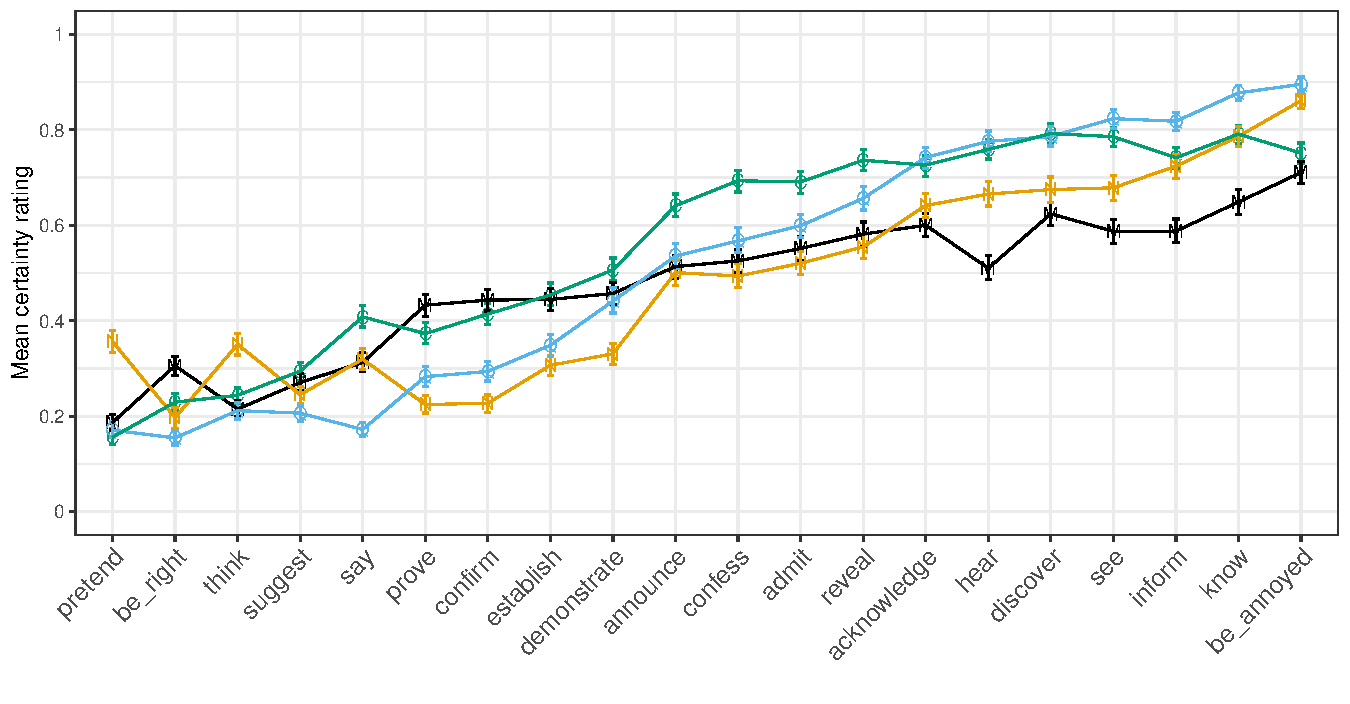
\includegraphics[width=\textwidth]{graphs/proj-by-both.pdf}}\vspace{-1.8\baselineskip}
	\caption{\small Mean certainty ratings by predicate and operator with 95\% bootstrapped confidence intervals. Embedding operator coded by letter and color:  \texttt{N} (orange): negation, \texttt{M} (black): modals, \texttt{C} (green): conditional antecedents, \texttt{Q} (blue): polar questions.}
	\label{fig:figure1}
\end{figure}

\begin{table}[h]
	\vspace{-1\baselineskip}\phantom{.}
	\centering
	\hspace{-1.3em}
	\begin{tabular}{p{.65\linewidth} p{.31\linewidth}}
		\scalebox{.75}{
			\begin{tabular}{llrrrr}
				Model & & Estimate & Std. Error & t-value\\
				\midrule
				\#1 & Intercept: \emph{question} & 0.51 & 0.01 & 44.78 & ***\\
				& operator: conditional & 0.05 & 0.01 & 5.30 & ***\\
				& operator: modal & -0.04 & 0.01 & -4.45 & ***\\
				& operator: negation & -0.03 & 0.01 & -4.67 & ***\\
				\midrule
				\#2 & Intercept: \emph{\bf be annoyed}/negation & 0.87 & 0.01 & 79.86 & ***\\
				& operator: conditional & -0.12 & 0.02  & -7.36 & ***\\
				& operator: modal & -0.16 & 0.02  & -10.01 & ***\\
				& operator: question & 0.02 & 0.01 & 1.72 & n.s.\\
				\midrule
				\#3 & Intercept: \emph{\bf discover}/negation & 0.68 & 0.01 & 62.70 & ***\\
				& operator: conditional & 0.11 & 0.02 & 7.11 & ***\\
				& operator: modal & -0.06 & 0.02 & -3.63 & ***\\
				& operator: question & 0.10 & 0.01 & 7.08 & ***\\
				\midrule
				\#4 & Intercept: \emph{\bf know}/negation & 0.79 & 0.01 & 72.97 & ***\\
				& operator: conditional & 0.00 & 0.02 & -0.06 & n.s.\\
				& operator: modal & -0.14 & 0.02 & -9.18 & ***\\
				& operator: question & 0.08 & 0.01 & 5.67 & ***\\
				\bottomrule
			\end{tabular}
		}
		&
		\parbox{\linewidth}{\caption{\small Excerpt of the output from three linear mixed effects models; \textbf{\#1} has fixed effects of operator; random effects: participant and item intercepts, \textbf{\#2-4} have fixed effect: operator, predicate, and their interaction; random effect: participant intercepts.
		Models were fit with \texttt{lme4, lmertest} in \texttt{R}. Models \textbf{\#2--4} also had at least $34$ highly significant interaction terms of \texttt{operator} and \texttt{predicate} with $p < 0.001$ (not shown here).}\label{t:models}}

	\end{tabular}
\end{table}

\hspace{-2.7em}
	\begin{minipage}{\textwidth}\centering
	\begin{tabular}{p{.235\linewidth} p{.235\linewidth} p{.235\linewidth} p{.235\linewidth}}
		\parbox{\linewidth}{\centering (a) \textbf{Negation high}\\
		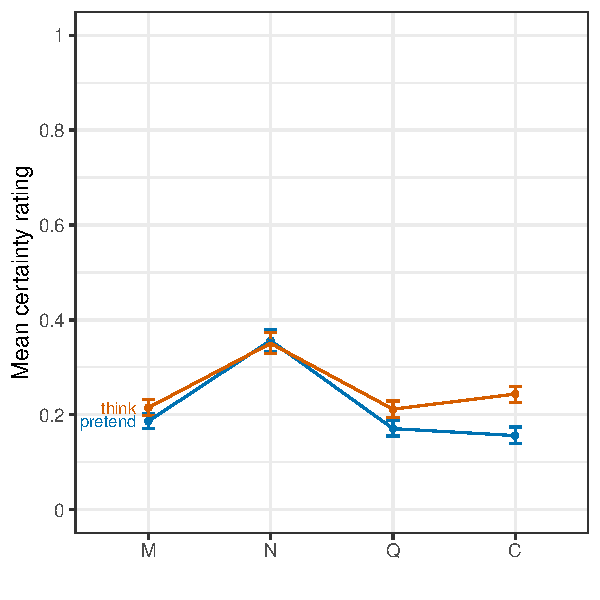
\includegraphics[width=.26\textwidth]{graphs/profile1.pdf}}
		&
		\parbox{\linewidth}{\centering (b) \textbf{Negation low}\\
		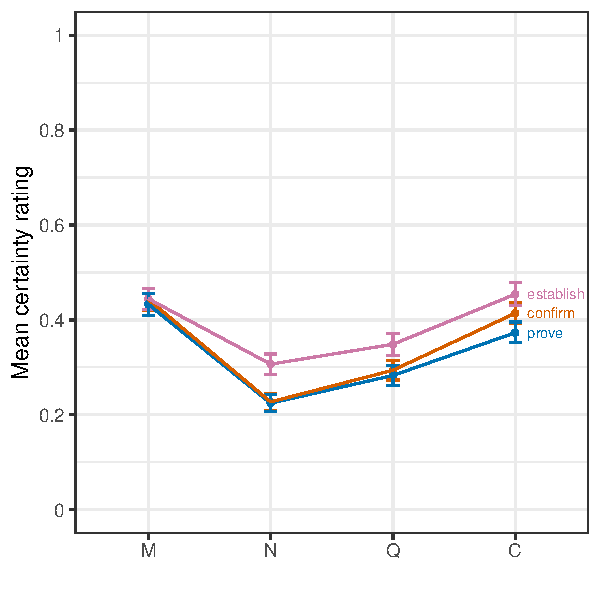
\includegraphics[width=.26\textwidth]{graphs/profile4.pdf}}
		&
		\parbox{\linewidth}{\centering (c) \textbf{Conditional high}\\
		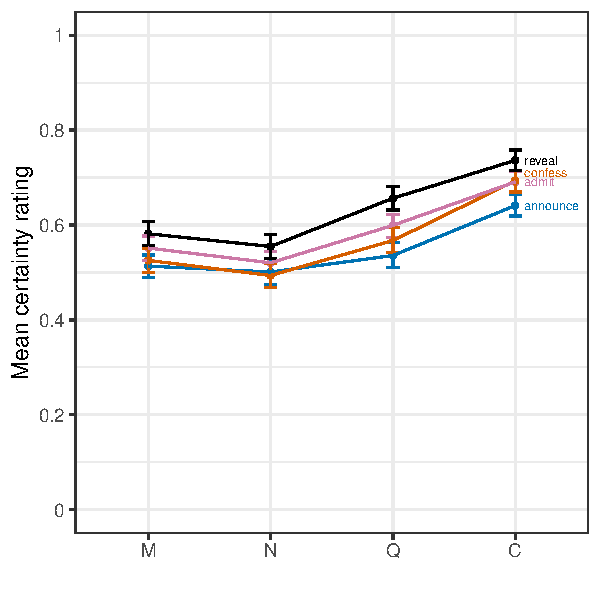
\includegraphics[width=.26\textwidth]{graphs/profile2.pdf}}
		&
		\parbox{\linewidth}{\centering (d) \textbf{Modal low}\\
		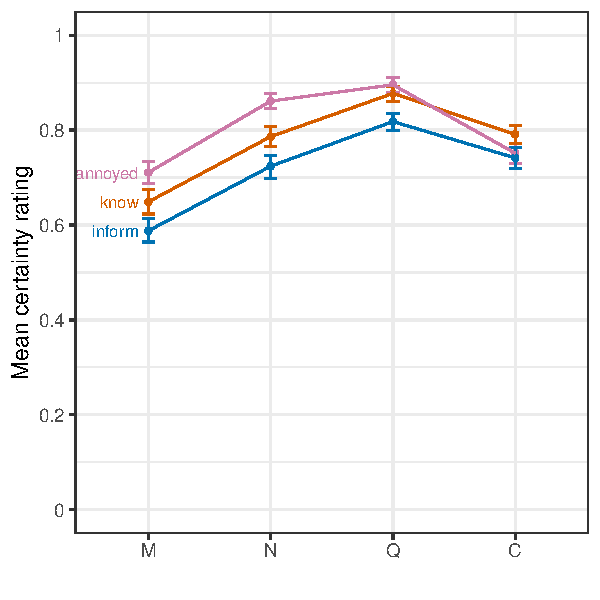
\includegraphics[width=.26\textwidth]{graphs/profile5.pdf}}
	\end{tabular}
\end{minipage}

\vspace{-.4\baselineskip}
\noindent \small Figure 2: \small Mean certainty ratings by operator (\texttt{M}: Modal, \texttt{N}: Negation, \texttt{Q}: Polar Question, \texttt{C}: Conditional antecedent) with 95\% bootstrapped confidence intervals, for some groups of predicates (\lq predicate patterns\rq).

% \begin{figure}[h]
% 	\hspace{-2.5em}
	
% 	\vspace{-\baselineskip}
% 	% \caption{Mean certainty-ratings by operator for four predicate patterns in our data.}
% 	\label{fig:figure2}
% \end{figure}

\newpage


% \bibliography{../bibliography.bib}
\bibliography{../projective-content.bib}

\end{document}